%!TEX root = nextndnvideo-tr.tex
\section{implementation} % (fold)
\label{sec:implementation}
Next-NDNVideo is developed using Consumer / Producer API over NDN. This API is an modification version of ndn-cxx library and requires NFD running to forward interests. To compact with Consumer / Producer API and NFD, the project is also written in C++. We use Gstreamer 1.4.3 (other branch not tested) to process media. The supporting platform is UNIX-Like such as Mac OS and Linux. We will explain the implementation details about Live Streaming and Prerecorded respectively.
\begin{figure}[htbp]
  \centering
  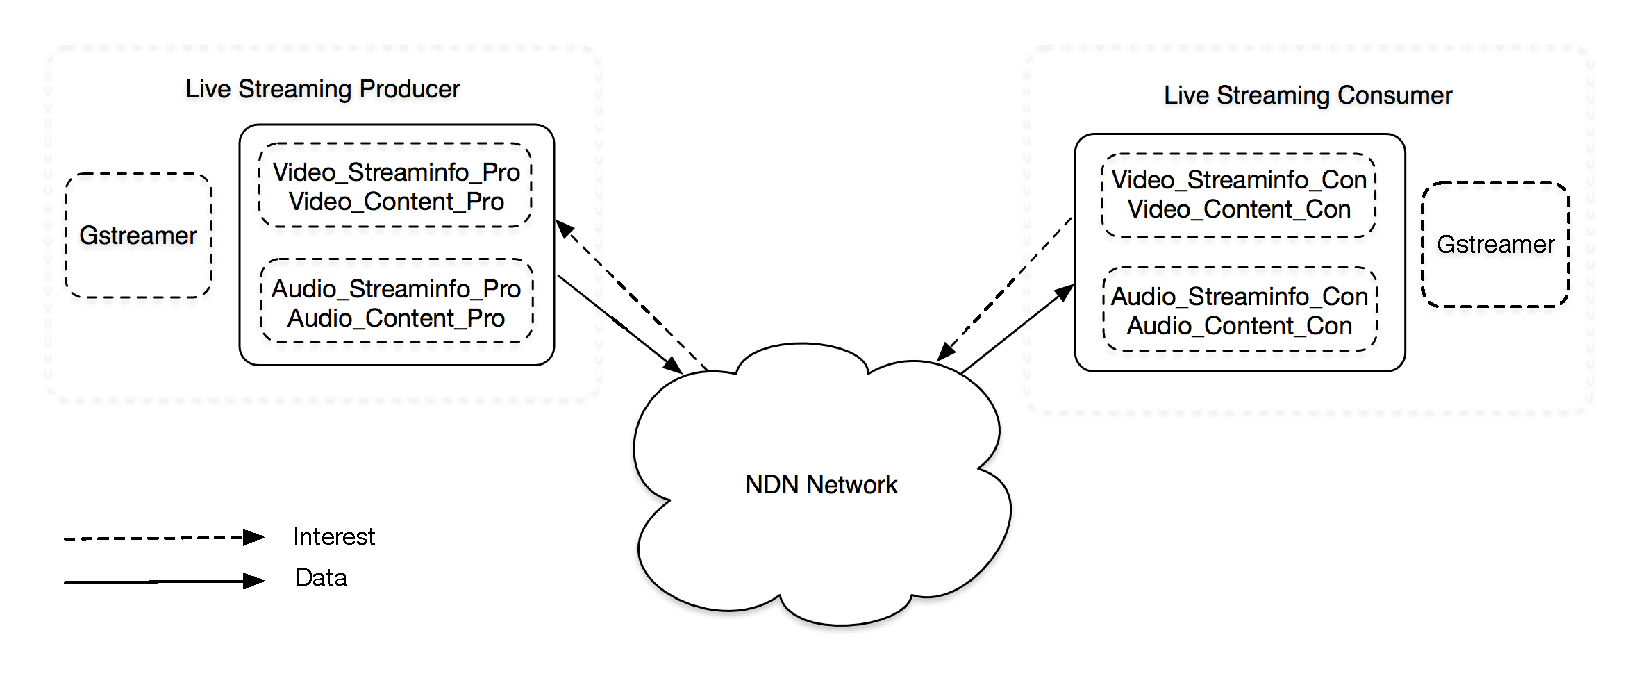
\includegraphics[scale=0.3]{live_arch}
  % \vspace{-0.3cm}
  \caption{Live Streaming Architecture}
  \label{fig:live_arch}
  %\vspace{-0.2cm}
\end{figure}

\subsection{Live Streaming}
The architecture of Live Streaming is shown as Figure~\ref{fig:live_arch}. It has four producers: video stream information producer, video content producer, audio stream information producer and audio content producer. Before the consumer asks for the true video data, it must fetch the live stream information to set up the Gstreamer playing pipeline. The stream information includes frame rate, width, height, stream format and so on. For Live streaming, to inform consumer of the starting frame number, the producer also need to produce the latest frame number if requested. The video and audio are produced and consumed separately, so they must be in separate thread. In both (producer and consumer) side, the Gstreamer should keep running in the background, so Gstreamer needs another thread. 

[To conclude, in each side we have three threads running at the same time. Components inside one black dotted rectangle belong to the same thread.] ------- have problems! now the consumer has video and audio running in the same thread, and boost scheduler will schdule the consume process every video or audio interval according to the video or audio frame rate. 

The following part will describe some details about media processing, the data retrieval protocols we use and the pseudo code.
\subsubsection {Media Precessing}
\paragraph {Producer}
The producer will capture video from camera and audio from microphone, then produce them frame by frame. The progressing detail is shown as Figure~\ref{fig:live_detail}.

\begin{figure*}%[htbp]
  \centering
  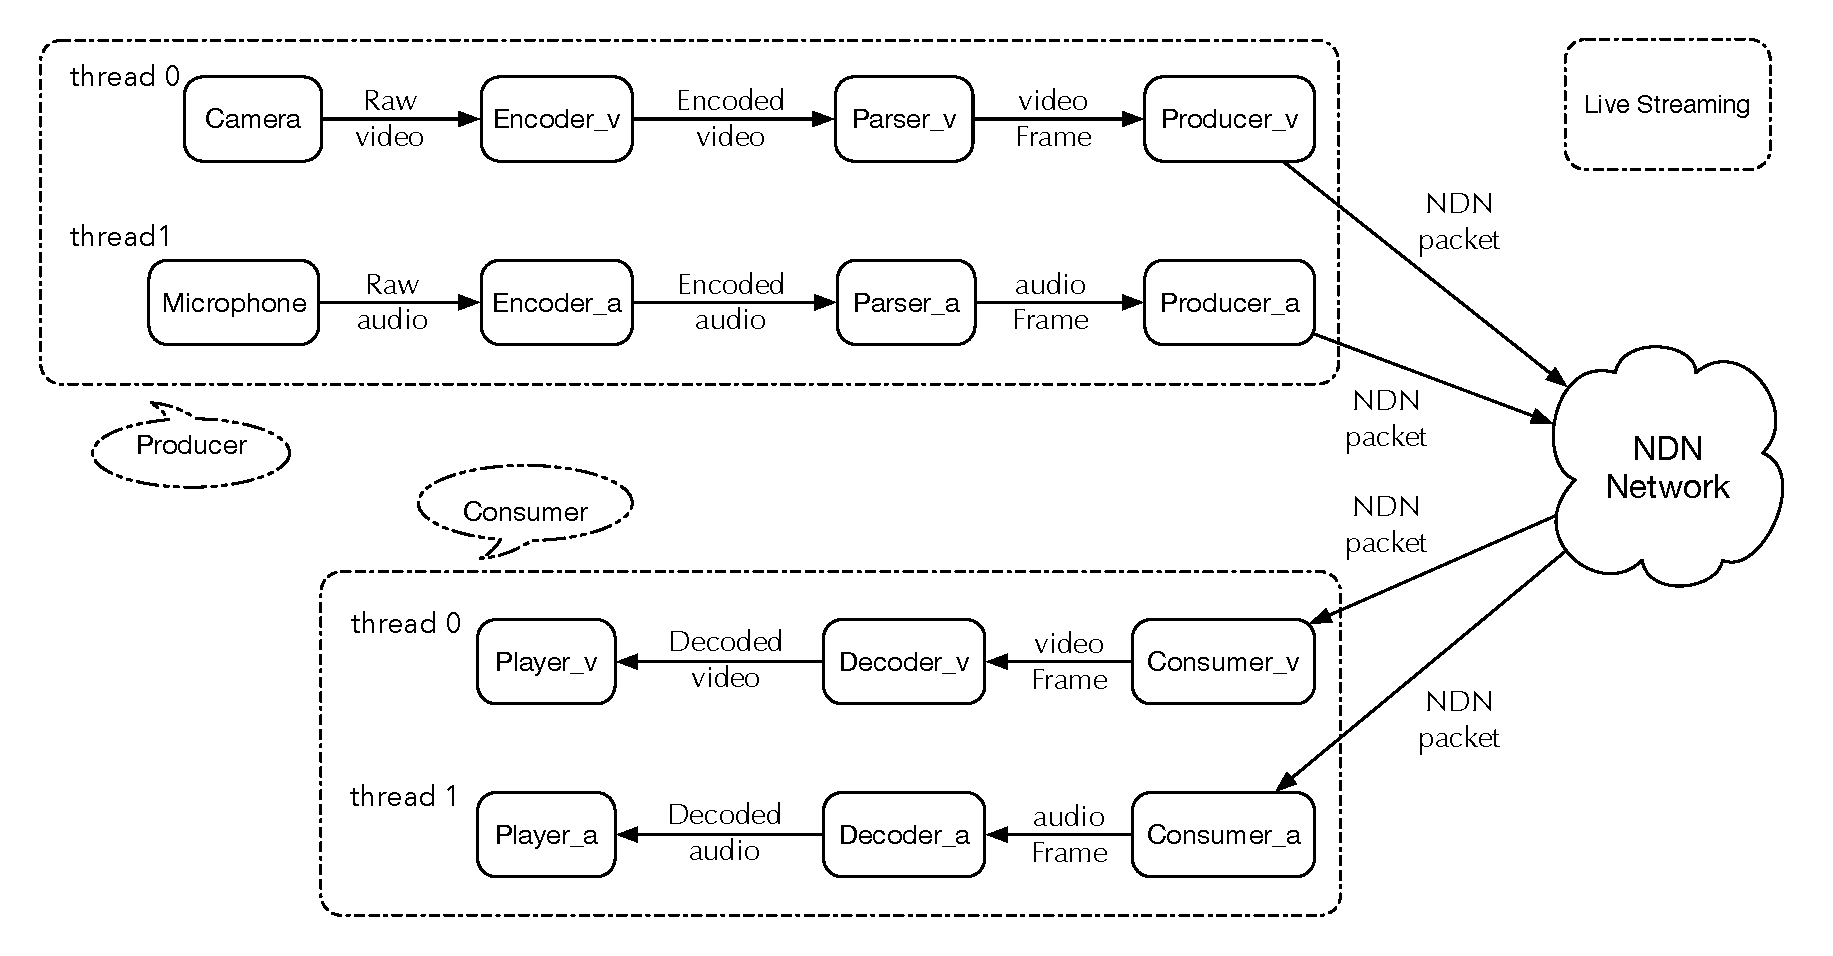
\includegraphics[scale=0.55]{live_detail}
  % \vspace{-0.3cm}
  \caption{Live Streaming Media Processing}
  \label{fig:live_detail}
  %\vspace{-0.2cm}
\end{figure*}

The raw video pictures captured by camera would be transferred to \textit{Encoder\_v} component and will be encoded into \textit{H264} format. Then the encoded video is transmitted into \textit{Parser\_v} to be parsed into frames (\textit{B, P or I frame}). The last component is the \textit{Producer\_v}, which is in charge of producing video frame by frame.

For audio, the microphone will capture the audio then push the raw audio into \textit{Encoder\_a}. The encoder component will encode the raw audio into \textit{AAC} format. The encoded audio stream will be transferred to \textit{Parser\_a} to get parsed then passed to \textit{Producer\_a} component. Finally, this audio producer will produce the audio frame by frame.

\paragraph {Consumer}
The consumer also processes video and audio separately.

For video, the \textit{Consumer\_v} component keeps sending interests to fetch the video data. And it will get data retrieved frame by frame. Then the video frame will be thrown to the \textit{Decoder\_v} to get decoded into the format which the \textit{Player\_v} can play it back.
For audio, the \textit{Consumer\_a} component fetches the audio data by sending audio interests. The retrieved audio frame will be transferred to \textit{Decoder\_a} to get decoded. The decoded audio will be sent to \textit{Player\_a}. At the end, the \textit{Player\_v} and \textit{Player\_a} should play video and audio together.

\paragraph {Synchronization between video and audio}
\label{par:sync}
Since we process video and audio separately, it is a vital problem to keep them synced. Gstreamer can handle the synchronization for us in this way:

When video and audio are captured, they are timestamped by the Gstreamer. The time information will be recorded in \textit{GstBuffer} data structure which Gstreamer used to contain media data. This time information will also be transferred along with video or audio frame. Then when the consumer fetches the video or audio frame separately. The video and audio frames will be pushed into the same \textit{GstQueue}. Gstreamer will extract the timestamps hiding in the video and audio frames, then play them back together according to the timestamps.

\subsubsection{Data Retrieval Protocol}
\paragraph{Streaminfo Retrieval} % (fold)
\label{par:streaminfo}
Because the stream information contains only one segment and will be fetched only one time (at the beginning of the playing back). We use \textbf{SDR} (\textit{Simple Data Retrieval}) to fetch the stream info for video and audio. Except for the basic stream information, the consumer also needs to obtain the current frame number the producer just produced. So that the frame consumer can start from this frame number and increase it one by one. To retrieve the latest stream information, \textit{Right\_Most\_Child} option should be set as TRUE.
\paragraph{Frames Retrieval} 
Considering about the situation of live streaming, the consumer part needs to keep the video and audio retrieving progress running all the time. The aim is to fetch all the segments inside one frame as soon as possible. The fetching process should NOT be blocked because of one segment missing. So we use \textbf{UDR} (\textit{Unreliable Data Retrieval}) for frames retrieval of living streaming. Then the consumer part should take care of the segments reassemble and ordering stuff.

\subsubsection{Pseudocode}

\begin{algorithm}%[hbtp]
\caption{Live video producer}
\label{alg:liveproducer}
\begin{algorithmic}[1]
\State $h_v \leftarrow $ \textbf{producer}(/ndn/ucla/livevideo/video/)
\State \textbf{setcontextopt}($h_v$, \textbf{cache\_miss}, \textit{ProcessInterest})
\State \textbf{attach}($h_v$)
\vspace{0.2cm}
	\While{\textit{TRUE}}
	\State $Name \textbf{ } suffix_v \leftarrow $ video frame number
	\State $content_v \leftarrow $ video frame captured from Camera
	\State \textbf{produce}($h_v$, $Name\textbf{ }suffix_v$, $content_v$)
	\EndWhile
\vspace{0.2cm}
\vspace{0.2cm}
\State $h_a \leftarrow $ \textbf{producer}(/ndn/ucla/livevideo/audio/)
\State \textbf{setcontextopt}($h_a$, \textbf{cache\_miss}, \textit{ProcessInterest})
\State \textbf{attach}($h_a$)
\vspace{0.2cm}
	\While{\textit{TRUE}}
	\State $Name \textbf{ } suffix_a \leftarrow $ audio frame number
	\State $content_a \leftarrow $ audio frame captured from mirophone
	\State \textbf{produce}($h_a$, $Name\textbf{ }suffix_a$, $content_a$)
	\EndWhile
\vspace{0.4cm}
\Function{ProcessInterest}{Producer \textbf{h}, Interest \textbf{i}}
  \If{\textit{NOT Ready}}
    \State $appNack \leftarrow $ \textbf{AppNack}($i$, \textbf{RETRY-AFTER})
    \State \textbf{setdelay}($appNack$, $estimated\_time$)
    \State \textbf{nack}($h$, $appNack$)
  \EndIf
   \If{\textit{Out of Date}}
    \State $appNack \leftarrow $ \textbf{AppNack}($i$, \textbf{NO-DATA})
    \State \textbf{nack}($h$, $appNack$)
  \EndIf
\EndFunction
\end{algorithmic}
\end{algorithm}

There are two situations we should consider carefully. The first one is that, because once the consumer started consuming frames, it will have no idea the about the current frame number which producer is producing. It may sometimes request for a frame number ahead of the producing. It is the producer's duty to inform the consumer about such knowledge. We introduce \textbf{NACK}(\textit{Negative Acknowledgment}) to handle such situation. 

For example, in Algorithm~\ref{alg:liveproducer} , when the interest asks for a piece of data not existing (out of date or not be produced yet), this will trigger the \textit{cache\_miss} callback function (\textit{Process\_Interest}). In that function, if the data was not produced (\textit{not\_ready}), the producer will set up an \textit{APPLICATION\_NACK} with \textit{PRODUCER\_DELAY} option for this interest together with the estimated delay time.

At the same time, although before the consumer starts to consume frames, it will ask for the current number. Such information may also go out of date because of the network delay. These out-of-date frames will never be produced again, because the streaming is live. When faced with such situation, the producer will simply send a \textbf{NACK} with \textit{NO-DATA} option.

\begin{algorithm}[hbtp]
\caption{Live video consumer}
\label{alg:liveconsumer}
\begin{algorithmic}[2]
\State $h_v \leftarrow $ \textbf{consumer}(/ndn/ucla/livevideo/video/, \textit{UDR})
%\State \textbf{setcontextopt}($h_v$, \textit{EMBEDDED\_MANIFESTS}, \textit{TRUE})
%\State \textbf{setcontextopt}($h_v$, \textbf{receive\_buffer\_size}, 1MB)
\State \textbf{setcontextopt}($h_v$, \textbf{new\_segment}, \textit{ReassambleVideo})
\vspace{0.2cm}
	\While{\textit{TRUE}}
	\State $Name \textbf{ } suffix_v \leftarrow $ video frame number
	\State \textbf{consume}($h_v$, $Name\textbf{ }suffix_v$)
	\State $framenumber ++$
	\EndWhile
\vspace{0.2cm}

\Function{ReassambleVideo}{Data \textbf{segment}}
    \State $content \leftarrow $ reassamble \textbf{segment}
    \If{\textit{Final\_Segment}}
		\State $video \leftarrow $ decode \textbf{content}
	   	\State Play $video$
	\EndIf
\EndFunction

\vspace{0.4cm}

\State $h_a \leftarrow $ \textbf{consumer}(/ndn/ucla/livevideo/audio/, \textit{UDR})
\State \textbf{setcontextopt}($h_a$, \textbf{new\_segment}, \textit{ReassambleAudio})
\vspace{0.2cm}
	\While{\textit{NOT EOS}}
	\State $Name \textbf{ } suffix_a \leftarrow $ audio frame number
	\State \textbf{consume}($h_a$, $Name\textbf{ }suffix_a$)
	\State $framenumber ++$
	\EndWhile
\vspace{0.2cm}

\Function{ReassambleAudio}{Data \textbf{segment}}
%   \State $video \leftarrow $ decode \textbf{content}
    \State $content \leftarrow $ reassamble \textbf{segment}
    \If{\textit{Final\_Segment}}
		\State $audio \leftarrow $ decode \textbf{content}
	   	\State Play $audio$
	\EndIf
\EndFunction
\end{algorithmic}
\end{algorithm}

\subsection{Pre-recorded Streaming}
\begin{figure}%[htbp]
  \centering
  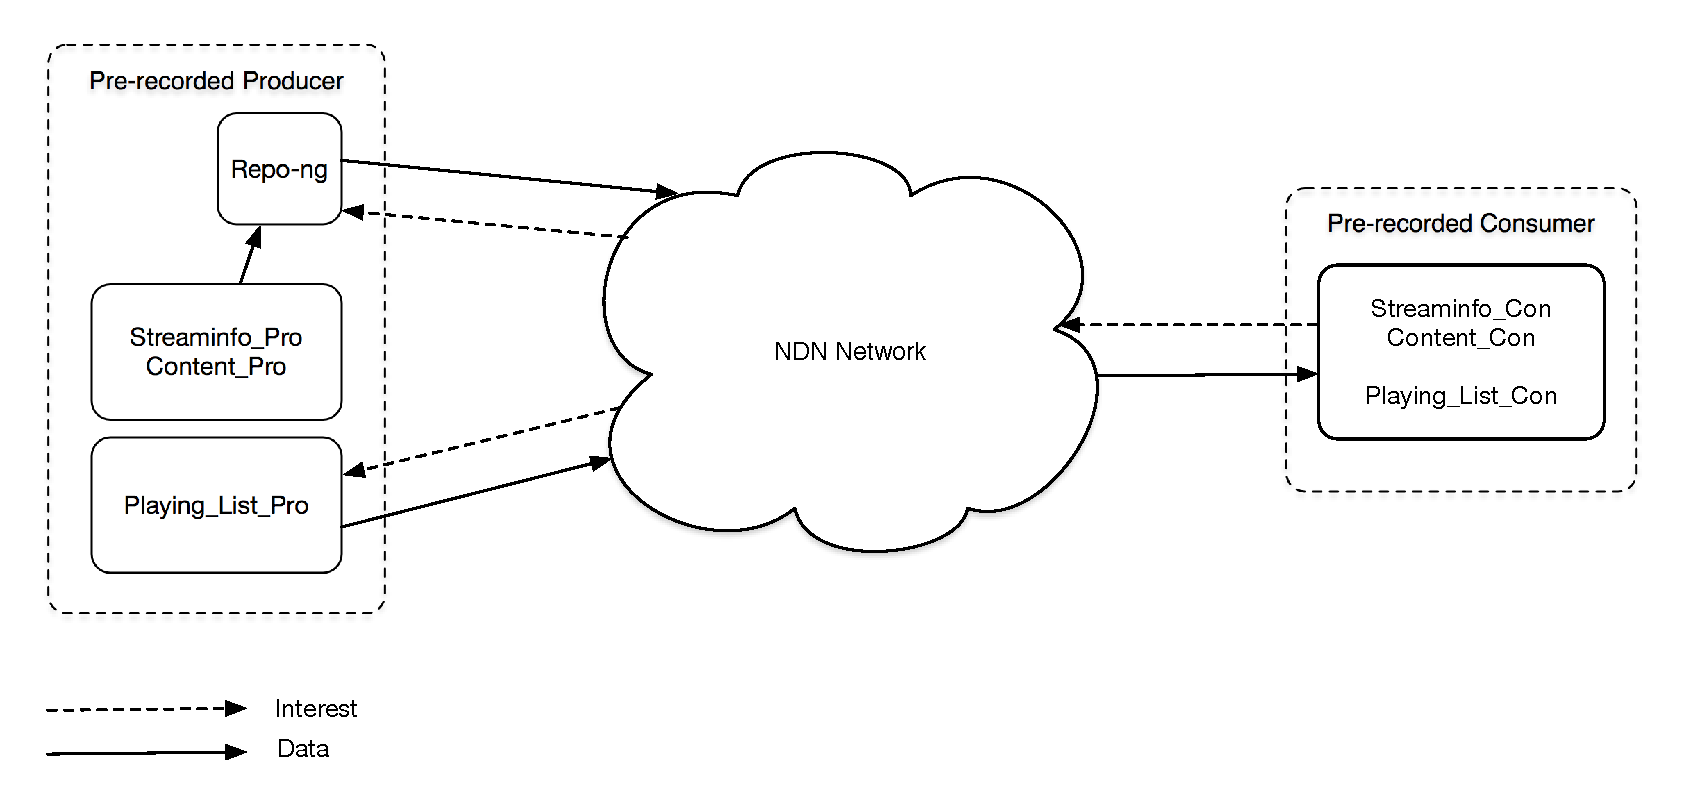
\includegraphics[scale=0.3]{record_arch}
  % \vspace{-0.3cm}
  \caption{Pre-recorded Streaming Architecture}
  \label{fig:record_arch}
  %\vspace{-0.2cm}
\end{figure}

The Pre-recorded Streaming architecture is slightly different from Live Streaming (Figure~\ref{fig:record_arch}). Firstly, \textbf{Repo-ng} is added in the producer side to provide the constant storage for video and audio data. Secondly, the playing list producer and consumer are introduced. This producer is to produce the playing list, which records the video names in one specific directory of producer. Because the video files could be added or deleted anytime, every time the producer detected the change of the directory, it will produce a new playing list with the same name except for appending a new timestamp. Figure~\ref{fig:list_naming} is one list naming example. 

\begin{figure}%[htbp]
  \centering
  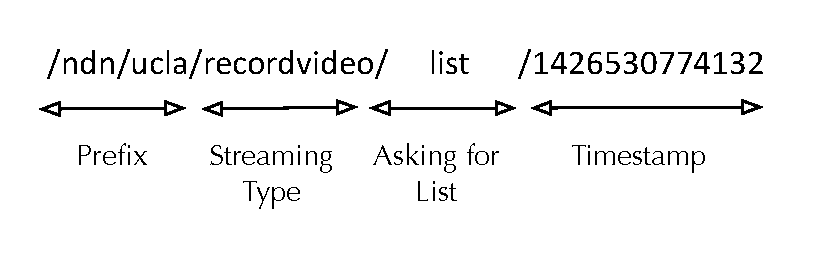
\includegraphics[scale=0.5]{list_naming}
  % \vspace{-0.3cm}
  \caption{Playing List Naming}
  \label{fig:list_naming}
  %\vspace{-0.2cm}
\end{figure}

The other two producers are almost the same with Live Streaming  One producer produces the stream information of the recorded video. The other takes charge of producing the frames, one slight difference is that we produce audio frames after video frames. This is to avoid the writing congestion of repo. The difference is that the stream info and frame data will be inserted into \textbf{Repo-ng}, but not attached to the NDN Network. Because different from live streaming, the pre-recorded video is permanent. Once the data was produced and the same data could be requested many times. However, for the live streaming, it just keeps producing and doesn't care about the data it produced several minutes ago. So the video file should be only produced once then written into Repo-ng and should not be produced again. The Repo-ng will respond to the interests. This can also relieve the producing pressure of producer.  

The consumer part should send interests to request the playing list in advance. Only after the consumer has the knowledge of all the files which producer has, it can ask for one specific video to play back. Same as live streaming, the pre-recorded video consumer also needs to retrieve the \textit{Streaminfo} of the video file to set up the playing pipeline of Gstreamer. Then the consumer keeps sending video and audio content retrieval interest with the frame number increased one by one. One difference from live streaming is that, the pre-recorded consumer must know the ending frame of the video file. So except for the basic information of pipeline, it should contain the final video and audio frame id. Then the consumer can know when to stop sending interests. On the contrary, the live streaming consumer just keep increasing the frame number until user close it. Because the video is alive and will be producing all the time. But the live streaming needs to obtain the current frame number to follow the step with the producer. The pre-recorded video consumer does not have this part.

[Another problem] ---- Should I mention the blocking style which we mimic youtube?

\subsubsection{Media Processing}

\begin{figure*}%[htbp]
  \centering
  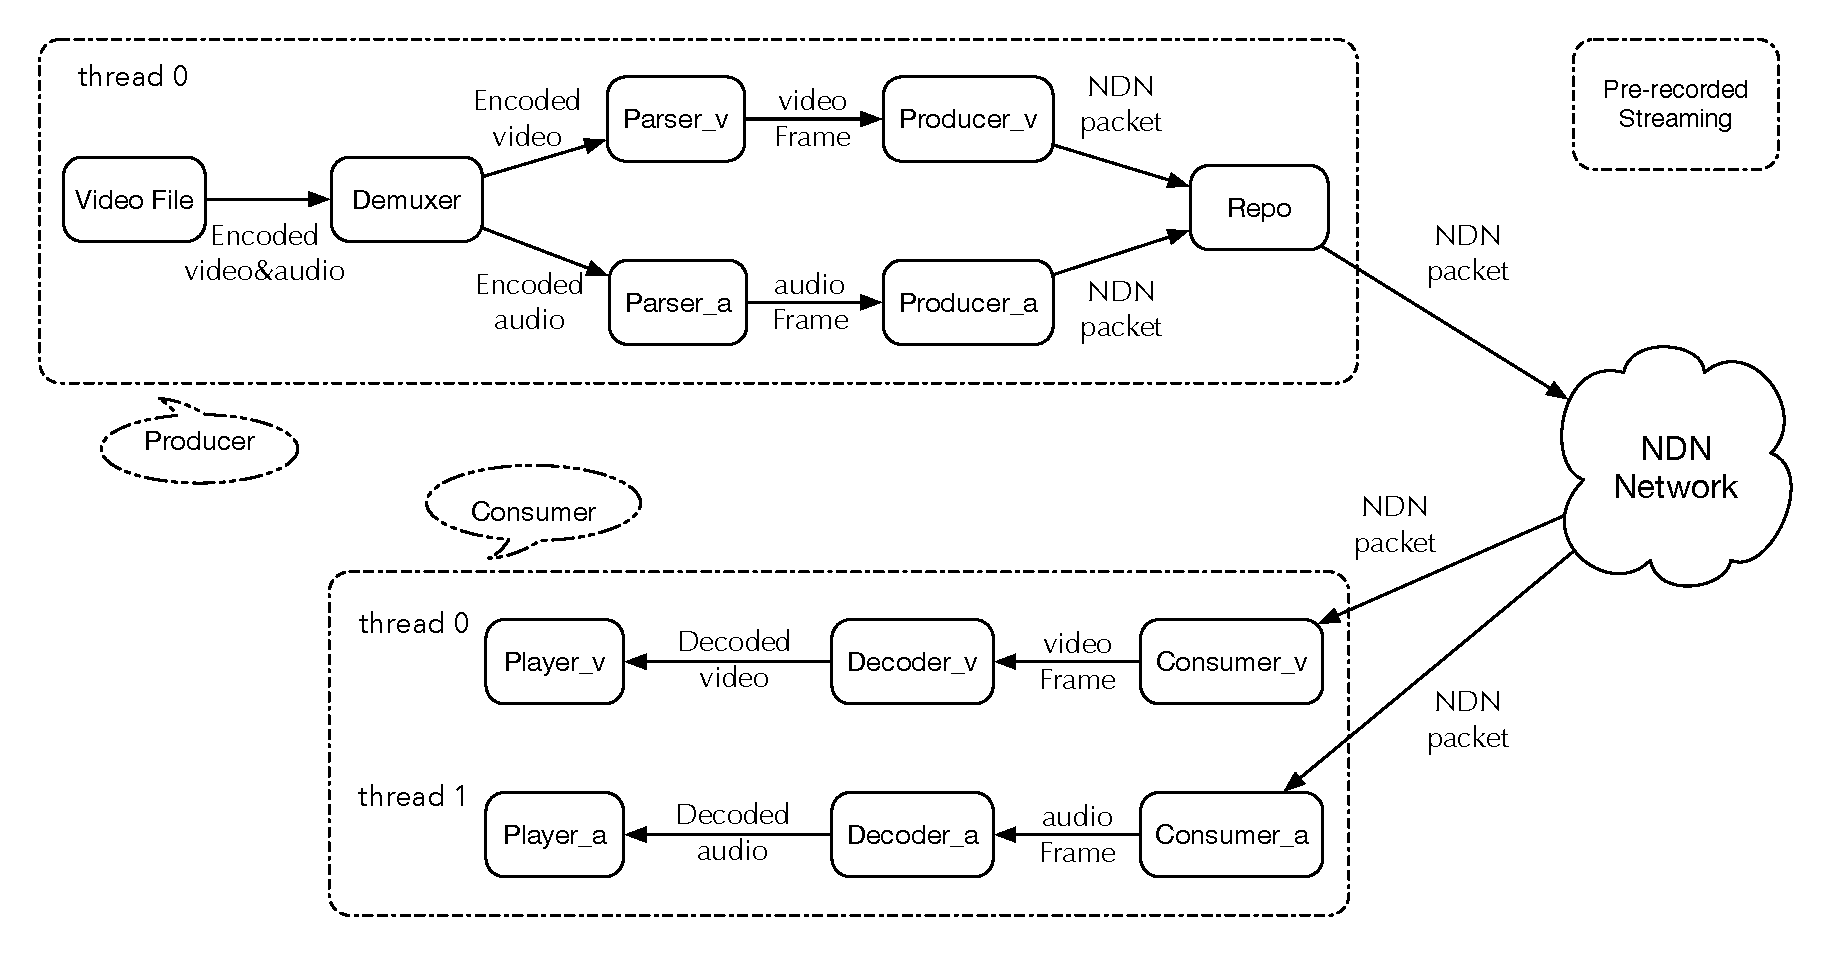
\includegraphics[scale=0.55]{record_detail}
  % \vspace{-0.3cm}
  \caption{Pre-recorded Streaming Media Processing}
  \label{fig:record_detail}
  %\vspace{-0.2cm}
\end{figure*}

The main difference from live streaming is the video source (Figure~\ref{fig:record_detail}). The pre-recorded video source is the video file. Gstreamer should first read video file then pass it to the \textit{Demuxer} component to separate video and audio stream. Because the video file is already encoded, so there is no \textit{Encoder} component here. The separate encoded video or audio is pushed into the \textit{Parser} to generate frames. The frames will be produced by Consumer / Producer API and inserted into \textit{Repo-ng}. The API will handle the segmentation automatically. The media processing of consumer part is the same with live streaming.

There also exists the synchronization problem between video and audio. As we describe above~\ref{par:sync}, the Gstreamer will handle the synchronization part as long as we give the video and audio frame correct timestamps. In live streaming, it is the capturing component who stamps the frames. In pre-recorded streaming, it is the \textit{Dumxer} who is responsible for time stamping. Once the media data flows through \textit{Dumxer}, this component will separate the video stream and audio stream according to their file type such as \textit{MP4} and adding the time information in each \textit{GstBuffer}.

\subsubsection{Data Retrieval}
Same with \textit{Streaminfo} tetrieval of live streaming, we use \textbf{SDR} to retrieve stream information and the playing list. We want to fetch the latest version of playing list, so we should set \textit{Right\_Most\_Child} option as TRUE as well.

However, for the frames retrieval, we should use \textbf{RDR} (\textit{Reliable Data Retrieval}). Because we can't stand any segment missing for the recorded video, we always want the good quality of video and audio. If the video segments are not received on time the \textit{Buffering} mechanism will be triggered. Only when Gstreamer accumulates enough video and audio frames (such as two seconds duration) it will continue to play back. Otherwise, it will be just paused until the buffer is full.

\subsubsection{Pseudocode}

[Say something here...]

\begin{algorithm}[hbtp]
\caption{Pre-recorded video publisher}
\label{alg:recordproducer}
\begin{algorithmic}[3]
\State $h_v \leftarrow $ \textbf{producer}(/ndn/ucla/recordvideo/video-1234/

video/)
\State \textbf{setcontextopt}($h_v$, \textbf{repo\_prefix}, \textit{/ndn/ucla/repo})
\vspace{0.2cm}
	\While{\textit{NOT EOF}}
	\State $Name \textbf{ } suffix_v \leftarrow $ video frame number
	\State $content_v \leftarrow $ video frame
	\State \textbf{produce}($h_v$, $Name\textbf{ }suffix_v$, $content_v$)
	%\State $framenumber ++$
	\EndWhile
\vspace{0.2cm}
\vspace{0.2cm}
\State $h_a \leftarrow $ \textbf{producer}(/ndn/ucla/recordvideo/video-1234/

audio/)
\State \textbf{setcontextopt}($h_a$, \textbf{repo\_prefix}, \textit{/ndn/ucla/repo})
\vspace{0.2cm}
	\While{\textit{NOT EOF}}
	\State $Name \textbf{ } suffix_a \leftarrow $ audio frame number
	\State $content_a \leftarrow $ audio frame
	\State \textbf{produce}($h_a$, $Name\textbf{ }suffix_a$, $content_a$)
	%\State $framenumber ++$
	\EndWhile
\end{algorithmic}
\end{algorithm}

\begin{algorithm}[hbtp]
\caption{Pre-recorded video consumer}
\label{alg:recordconsumer}
\begin{algorithmic}[4]
\State $h_v \leftarrow $ \textbf{consumer}(/ndn/ucla/recordvideo/video-1234/

video/, \textit{RDR})
%\State \textbf{setcontextopt}($h_v$, \textit{EMBEDDED\_MANIFESTS}, \textit{TRUE})
%\State \textbf{setcontextopt}($h_v$, \textbf{receive\_buffer\_size}, 1MB)
\State \textbf{setcontextopt}($h_v$, \textbf{new\_content}, \textit{ProcessVideo})
\vspace{0.2cm}
	\While{\textit{NOT EOS}}
	\State $Name \textbf{ } suffix_v \leftarrow $ video frame number
	\State \textbf{consume}($h_v$, $Name\textbf{ }suffix_v$)
	\State $framenumber ++$
	\EndWhile
\vspace{0.2cm}

\Function{ProcessVideo}{byte[] \textbf{content}}
   \State $video \leftarrow $ decode \textbf{content}
%   \State $audio \leftarrow $ decode \textbf{content}
   \State Play $video$
\EndFunction

\vspace{0.4cm}

\State $h_a \leftarrow $ \textbf{consumer}(/ndn/ucla/recordvideo/video-1234/

audio/, \textit{RDR})
\State \textbf{setcontextopt}($h_a$, \textbf{new\_content}, \textit{ProcessAudio})
\vspace{0.2cm}
	\While{\textit{NOT EOS}}
	\State $Name \textbf{ } suffix_a \leftarrow $ audio frame number
	\State \textbf{consume}($h_a$, $Name\textbf{ }suffix_a$)
	\State $framenumber ++$
	\EndWhile
\vspace{0.2cm}

\Function{ProcessAudio}{byte[] \textbf{content}}
%   \State $video \leftarrow $ decode \textbf{content}
   	\State $audio \leftarrow $ decode \textbf{content}
   	\State Play $audio$
\EndFunction
\end{algorithmic}
\end{algorithm}
% section implementation (end)